\section{Code, data, and reproducibility}
\label{app:code_and_data}

\paragraph{Code.} The JaxARC environment, all action and observation wrappers, the dataset parsers, the registration and subset-loading code, and the visualization utilities are released as anonymized open-source repositories for review:

\begin{itemize}
    \item \textbf{JaxARC environment:} \url{https://anonymous.4open.science/r/JaxARC-8788}
    \item \textbf{Baselines and experiment configurations:} \url{https://anonymous.4open.science/r/jaxarc-baselines-561F}
\end{itemize}

The baselines repository contains the Hydra configurations, the launcher used for the multi-algorithm sweep, the Stoix integration code, and the plotting scripts. Both repositories are MIT-licensed and will be de-anonymized at the camera-ready stage.

\paragraph{Datasets.} All datasets used in this paper are public. ARC-AGI-1 and ARC-AGI-2 are released under the Apache 2.0 license by their respective authors \citep{cholletMeasureIntelligence2019,cholletARCAGI2NewChallenge2025}; MiniARC is released under the Apache 2.0 license \citep{kimPlaygroundsAbstractionReasoning2022}; ConceptARC is released under the MIT license \citep{moskvichevConceptARCBenchmarkEvaluating2023}. JaxARC's \texttt{auto\_download} hook fetches each dataset from its upstream repository on first use; users are not required to pre-stage any data.

\paragraph{Reproducing the results.} The throughput benchmark, the multi-algorithm sweep, and the observation-wrapper diagnostic are each driven by Hydra configuration files in the baselines repository under \texttt{experiments/configs/}. The exact configuration filenames, command lines, software versions (Python 3.13.5, JAX 0.6.2, NumPy 2.3.1, Gymnasium 1.2.0), and per-run compute budgets used to produce every reported number are documented in the repositories' \texttt{README} files.

\section{Environment interface and implementation}
\label{app:environment_interface}

\subsection{Task and transition visualization}
\label{app:visualization}

JaxARC ships with four visualization modes (Figure~\ref{fig:viz_modes_appendix}). They render the working grid alongside relevant task context, action selections, and rewards, and are intended for qualitative analysis, debugging, and policy inspection. All renderers operate on host-side copies of the environment state, so they can be combined with any wrapper stack without affecting the compiled rollout.

\begin{figure}[htbp]
    \centering
    \begin{minipage}[c]{0.23\linewidth}
        \centering
        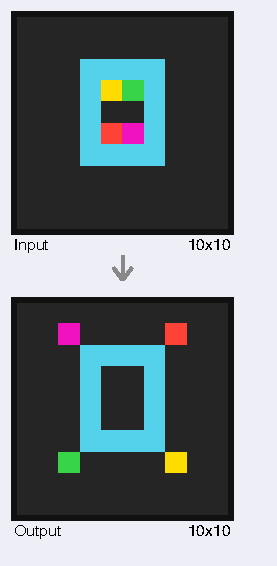
\includegraphics[width=\linewidth]{Figures/viz_task_pair.pdf}
        \small (a) Pair view
    \end{minipage}
    \hfill
    \begin{minipage}[c]{0.74\linewidth}
        \centering
        \begin{minipage}[b]{0.32\linewidth}
            \centering
            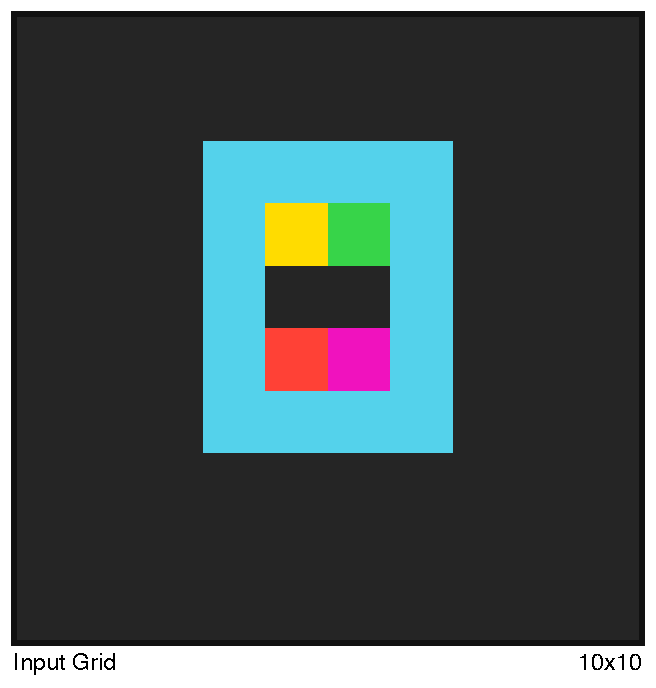
\includegraphics[width=\linewidth]{Figures/viz_single_grid.pdf}
            \small (b) Grid view
        \end{minipage}
        \hfill
        \begin{minipage}[b]{0.64\linewidth}
            \centering
            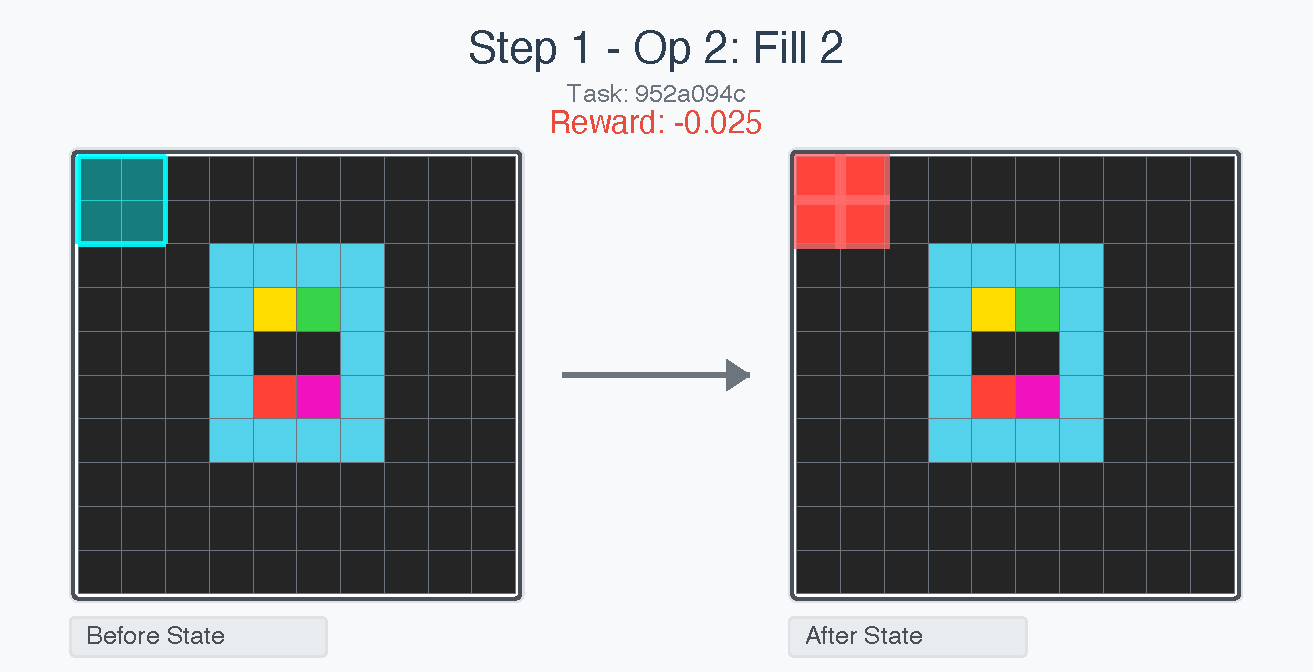
\includegraphics[width=\linewidth]{Figures/viz_rl_step.pdf}
            \small (c) Transition
        \end{minipage}

        \vspace{0.5em}

        \begin{minipage}[b]{0.98\linewidth}
            \centering
            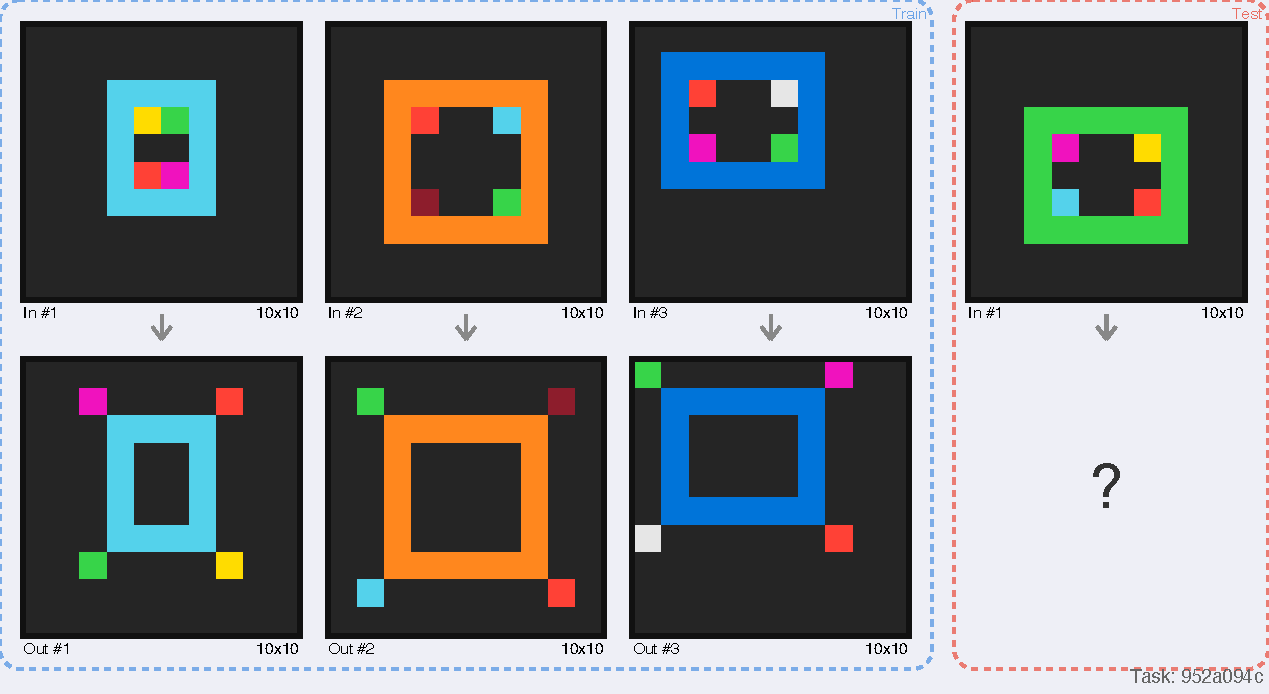
\includegraphics[width=\linewidth]{Figures/viz_complete_task.pdf}
            \small (d) Full task context
        \end{minipage}
    \end{minipage}
    \caption{Visualization modes in JaxARC. (a) A single input--output example. (b) A standalone grid. (c) A single RL step with action and reward annotations. (d) The complete task anatomy, showing support pairs and a held-out query.}
    \label{fig:viz_modes_appendix}
\end{figure}

\subsection{Internal data structures}
\label{app:data_structures}

JaxARC keeps a strict separation between immutable task data (\texttt{JaxArcTask}), static environment parameters (\texttt{EnvParams}), and the dynamic per-episode state (\texttt{State}). All three are Equinox PyTrees with statically-shaped leaves, so they can be freely passed through \texttt{jit}, \texttt{vmap}, and \texttt{pmap}. Table~\ref{tab:state_layout} lists the dynamic fields of \texttt{State}; the static parameters reside in \texttt{EnvParams} together with the stacked task buffer and the optional subset index view.

\begin{table}[htbp]
\centering
\caption{Dynamic per-episode state in JaxARC. All grids and masks are padded to the dataset's $H_{\max} \times W_{\max}$ canvas; counts apply to the active region defined by \texttt{working\_grid\_mask}.}
\label{tab:state_layout}
\scriptsize
\resizebox{\linewidth}{!}{%
\begin{tabular}{@{}lll@{}}
\toprule
\textbf{Field} & \textbf{Type / shape} & \textbf{Role} \\
\midrule
\texttt{working\_grid} & \texttt{int32[$H_{\max}, W_{\max}$]} & Current grid being edited (color values $0$--$9$) \\
\texttt{working\_grid\_mask} & \texttt{bool[$H_{\max}, W_{\max}$]} & Active cells of the working grid \\
\texttt{input\_grid}, \texttt{input\_grid\_mask} & same shapes & Original input grid for the active pair \\
\texttt{target\_grid}, \texttt{target\_grid\_mask} & same shapes & Target grid; masked to background in query mode \\
\texttt{selected} & \texttt{bool[$H_{\max}, W_{\max}$]} & Selection mask for the next operation \\
\texttt{clipboard} & \texttt{int32[$H_{\max}, W_{\max}$]} & Buffer for copy/paste operations \\
\texttt{step\_count} & \texttt{int32} & Current step within the episode \\
\texttt{task\_idx}, \texttt{pair\_idx} & \texttt{int32} & Indices into the task buffer \\
\texttt{allowed\_operations\_mask} & \texttt{bool[$35$]} & Currently enabled operations \\
\texttt{similarity\_score} & \texttt{float32} & Match between working and target grid \\
\texttt{key} & \texttt{uint32[$2$]} & Per-environment PRNG key \\
\bottomrule
\end{tabular}
}
\end{table}

The task buffer is a single stacked PyTree of \texttt{JaxArcTask} fields, prepared on the host and transferred to the device once. Each task entry stores up to \texttt{max\_train\_pairs} support pairs (default 10) and \texttt{max\_test\_pairs} query pairs (default 3), together with their boolean masks and an integer task identifier. Subset selection is implemented as an \texttt{int32} \texttt{subset\_indices} array that gathers from the full buffer, so subsets do not require recompilation.

\subsection{Reset and transition semantics}
\label{app:reset_and_step}

The compiled \texttt{reset} samples a task index from the active subset, samples a pair index uniformly from the available support or query pairs, and constructs the initial \texttt{State} via the working-grid initializer (Section~\ref{app:grid_init}). The \texttt{step} function performs four operations: (i) operation validation against the active operation profile, (ii) execution of the selected grid operation, (iii) computation of the new similarity score against the target grid, and (iv) emission of a Stoa \citep{toledoStoaJAXnativeInterface2025} \texttt{TimeStep} with one of three step types.

\begin{itemize}
    \item \texttt{TERMINATED} when the agent submits (operation $34$), regardless of whether the submission is correct.
    \item \texttt{TRUNCATED} when \texttt{step\_count} reaches \texttt{max\_episode\_steps} without a submission.
    \item \texttt{MID} otherwise.
\end{itemize}

The discount factor is set to $0$ on \texttt{TERMINATED} and \texttt{TRUNCATED} steps and to $1$ on \texttt{MID} steps. The episode mode (\texttt{train} vs \texttt{test}) is carried inside \texttt{EnvParams} rather than \texttt{State}, which allows the same compiled environment to be re-used for both visible-target rollouts and hidden-target evaluation by swapping \texttt{EnvParams}.

\paragraph{Reward components.} The submit-aware reward used by every profile is the sum
\begin{equation*}
    r_t = \alpha \,\Delta s_t \cdot \mathbb{1}[\text{train}]\;+\; c_{\text{step}}\;+\; b_{\text{succ}}\,\mathbb{1}[\text{submit} \wedge s_t = 1]\;+\; p_{\text{unsolved}}\,\mathbb{1}[\text{submit} \wedge s_t < 1],
\end{equation*}
where $s_t$ is the similarity score after the step, $\Delta s_t = s_t - s_{t-1}$ is its improvement, and the constants $\alpha, c_{\text{step}}, b_{\text{succ}}, p_{\text{unsolved}}$ are taken from the active reward profile (Section~\ref{app:reward_config}). Similarity shaping is automatically disabled in evaluation mode, where $\Delta s_t$ is multiplied by $\mathbb{1}[\text{train}]=0$, leaving only the step penalty, success bonus, and unsolved penalty.

\subsection{Grid similarity score}
\label{app:similarity}

Similarity is computed against the target grid's active region. Let $\mathcal{T}$ be the set of cells with \texttt{target\_grid\_mask}$=$true; the similarity is
\begin{equation*}
    s = \frac{1}{|\mathcal{T}|}\sum_{(i,j) \in \mathcal{T}} \mathbb{1}\!\left[\text{working}_{ij} = \text{target}_{ij}\;\wedge\;\text{working\_grid\_mask}_{ij}\right],
\end{equation*}
with $s = 1$ when both grids are empty and $s = 0$ when the target is empty but the working grid contains content. This definition penalizes both content mismatches and size mismatches: cells outside the target's active region or outside the working grid's active region count as incorrect, so an oversized or undersized submission cannot reach $s=1$. A solved episode requires $s=1$ at the moment the agent emits the \texttt{SUBMIT} operation; truncation alone never grants the success bonus.

\subsection{Working-grid initialization strategies}
\label{app:grid_init}

The initial working grid is sampled from a configurable mixture of four strategies. Weights need not sum to one; they are renormalized at compile time. Table~\ref{tab:grid_init} lists the strategies and their behavior. The baseline experiments use \texttt{demo\_weight}$=1.0$ (the remaining weights set to zero), which reproduces the standard ARC formulation in which the agent edits the input grid into the target output. Permutation, empty, and random initializers are intended for curriculum, robustness, and pre-training studies that go beyond the scope of this paper.

\begin{table}[htbp]
\centering
\caption{Working-grid initialization strategies. The agent is assigned one strategy per episode using the configured weights.}
\label{tab:grid_init}
\scriptsize
\resizebox{\linewidth}{!}{%
\begin{tabular}{@{}lll@{}}
\toprule
\textbf{Mode} & \textbf{Source} & \textbf{Behavior} \\
\midrule
\texttt{demo} & A randomly sampled support pair input & Standard ARC editing setup \\
\texttt{permutation} & Demo input with a random rotation, reflection, or color remap & Synthetic augmentation \\
\texttt{empty} & Padded zero grid with the dataset's grid mask & Pure ``construct from scratch'' setting \\
\texttt{random} & Sparse or dense Bernoulli pattern over the active mask & Robustness / noise probing \\
\bottomrule
\end{tabular}
}
\end{table}

\subsection{API usage examples}
\label{app:usage}

JaxARC follows the stateless API used by JAX environment libraries: random state is carried through explicit PRNG keys, and the environment state is a PyTree passed into and returned from each transition. Listing~\ref{lst:minimal_api} shows a single-task loop. Listing~\ref{lst:batched_api} shows the same reset and step functions under \texttt{vmap}.

\begin{lstlisting}[style=jaxarcpython, caption={Minimal transition loop for a single task.}, label={lst:minimal_api}]
import jax
from jaxarc import make

# Initialize environment and static parameters
env, env_params = make("Mini-Most_Common_color_l6ab0lf3xztbyxsu3p")

# Stateless reset
key = jax.random.PRNGKey(0)
state, timestep = env.reset(key, env_params=env_params)

action = env.action_space(env_params).sample(key)
state, timestep = env.step(state, action, env_params=env_params)
\end{lstlisting}

\begin{lstlisting}[style=jaxarcpython, caption={High-throughput vectorization using \texttt{vmap}.}, label={lst:batched_api}]
num_envs = 1024
keys = jax.random.split(jax.random.PRNGKey(0), num_envs)

# Batch the reset logic
reset_one = lambda k: env.reset(k, env_params=env_params)
states, timesteps = jax.jit(jax.vmap(reset_one))(keys)

# Batch the step logic
step_one = lambda s, a: env.step(s, a, env_params=env_params)
actions = jax.vmap(env.action_space(env_params).sample)(keys)
states, timesteps = jax.jit(jax.vmap(step_one))(states, actions)
\end{lstlisting}

\section{Datasets and task subsets}
\label{app:datasets}

JaxARC partitions the ARC problem space into datasets, each managed by a parser and registry entry. The parsers preserve ARC's native grid-size range ($1 \times 1$ to $30 \times 30$) while padding task tensors into fixed-shape accelerator buffers. A scenario selects the active task subset before compilation, for example \texttt{AGI1-entry} or \texttt{Concept-Count}. This keeps the compiled transition shape static while allowing the benchmark to report by task family.

\subsection{ARC-AGI-1 groups}
\label{app:arcagi_subsets}

For the ARC-AGI-1 sweep, we adopted the task tiers defined by the ARC-Game project at \url{https://github.com/volotat/ARC-Game/blob/main/tasks/levels.json}. While these labels provide a useful heterogeneous reporting structure, we emphasize that they are subjective and have not been formally calibrated for difficulty. Table~\ref{tab:agi1_subset_counts} lists the counts for each label used in this work; counts match the YAML subset files shipped with the JaxARC baseline configurations.

\begin{table}[htbp]
\centering
\caption{ARC-AGI-1 groupings used for benchmarking. Task counts are based on subjective ARC-Game labels.}
\label{tab:agi1_subset_counts}
\small
\begin{tabular}{@{}lr@{}}
\toprule
\textbf{Grouping} & \textbf{Tasks} \\
\midrule
\texttt{entry} & 33 \\
\texttt{easy} & 304 \\
\texttt{medium} & 263 \\
\texttt{hard} & 66 \\
\texttt{multiple\_solutions} & 33 \\
\texttt{tedious} & 73 \\
\bottomrule
\end{tabular}
\end{table}

\subsection{ConceptARC concept groups}
\label{app:concept_mini}

The ConceptARC benchmark is organized into concept groups that isolate specific spatial or logical rules. Our main baseline figure focuses on six representative groups: AboveBelow, Center, CleanUp, CompleteShape, Copy, and Count. The full 16-group breakdown is reported in Appendix~\ref{app:extended_baselines}.

\subsection{Extensibility and custom subsets}
\label{app:extensibility}

JaxARC is designed for easy extension to new task families and curated subsets. The \texttt{make} function provides a unified interface for instantiating environments from predefined groups, custom YAML files, or individual tasks.

\paragraph{Predefined subsets.}
To facilitate standard benchmarking, common task groupings are predefined and available immediately:
\begin{itemize}
    \item \textbf{ConceptARC:} All 16 concept groups are registered as subsets (e.g., \texttt{make("Concept-AboveBelow")}).
    \item \textbf{ARC-AGI:} The standard splits are available as \texttt{make("AGI1-train")} and \texttt{make("AGI1-eval")}.
    \item \textbf{Single tasks:} Any individual task can be isolated by appending its ID to the dataset key (e.g., \texttt{make("Mini-l6ab0lf3...")}). This is particularly useful for debugging specific reasoning failures.
\end{itemize}

\paragraph{YAML-based subsets.}
A common pattern for creating reproducible benchmarks is to define a subset in a YAML file. These files should be placed in the project configuration directory under \texttt{configs/env/jaxarc/subsets/\{Dataset\}/\{name\}.yaml}. Once the file is saved, the subset can be instantiated using the hyphenated identifier (e.g., \texttt{make("AGI1-my\_benchmark")}). Library users should first call \texttt{load\_all\_subsets\_for\_dataset("AGI1")} to discover these files at process start-up.

\paragraph{Programmatic registration.}
Subsets can also be registered at runtime without modifying the file system. This is useful for implementing curriculum learning or dynamically generating task groups during an experiment.

\begin{lstlisting}[style=jaxarcpython, caption={Programmatic subset registration and single-task instantiation.}]
from jaxarc.registration import register_subset, make

# 1. Register a custom task group
my_tasks = ["task_id_1", "task_id_2"]
register_subset("Mini", "custom_group", my_tasks)
env, params = make("Mini-custom_group")

# 2. Instantiate a single specific task
env, params = make("Mini-Most_Common_color_l6ab0lf3xztbyxsu3p")
\end{lstlisting}

\paragraph{Zero-config initialization and auto-download.}
To minimize setup friction, JaxARC includes an \texttt{auto\_download} parameter in the \texttt{make} function. When set to \texttt{True}, the environment registry detects if the required dataset files are missing from the local cache, fetches them from the official upstream repository, and organizes the files in the appropriate local directory before proceeding with environment creation.

\begin{lstlisting}[style=jaxarcpython, caption={Zero-config instantiation with automatic dataset acquisition.}]
from jaxarc.registration import make

# Automatically downloads AGI1 tasks if not present locally
env, params = make("AGI1-entry", auto_download=True)
\end{lstlisting}

For ARC-AGI datasets the registry performs cross-split lookups automatically: if a task ID is requested but not found in the current split (e.g., \texttt{train}), the system attempts to locate it in the opposite split (\texttt{evaluation}) before reporting an error. This makes it possible to define a custom subset that mixes IDs from both standard splits without writing a custom parser.

\section{Configuration surface}
\label{app:configuration_surface}

JaxARC exposes the main experimental degrees of freedom as explicit configuration axes. Table~\ref{tab:hydra_config_surface} summarizes these axes and the specific values used in our multi-algorithm baselines.

\begin{table}[htbp]
\centering
\caption{Experimental configuration surface in JaxARC.}
\label{tab:hydra_config_surface}
\scriptsize
\resizebox{\linewidth}{!}{%
\begin{tabular}{@{}lll@{}}
\toprule
\textbf{Axis} & \textbf{Value(s) used in this paper} & \textbf{Description} \\
\midrule
Dataset & ARC-AGI-1, ConceptARC, MiniARC & Source of raw JSON tasks \\
Scenario & e.g., \texttt{AGI1-entry}, \texttt{Concept-Count} & Active task subset selector \\
Action mode & \texttt{point} & Parameterization of the selection mask \\
Operation profile & \texttt{raw} (unless specified otherwise) & Allowed set of editing operations \\
Observation stack & answer, input, contextual & Configured grid channels for the policy \\
Reward profile & balanced & Shaping and submission rewards \\
Episode limit & 100 steps & Maximum edits before truncation \\
Grid initializer & \texttt{demo} (weight $1.0$) & Working grid copies the support input \\
Evaluation schedule & 20 intervals, 32 episodes each & Periodic monitoring during training \\
\bottomrule
\end{tabular}
}
\end{table}

\section{Interface and reward design}
\label{app:action_reward_config}

\subsection{Action wrappers}
\label{app:action_config}

The environment core receives an operation ID and a selection mask. To keep the action space tractable for discrete RL, we provide wrappers that simplify this interface. The \texttt{point} wrapper, used in our baselines, represents an action as $(\texttt{op}, \texttt{row}, \texttt{col})$, while the \texttt{bbox} wrapper accepts $(\texttt{op}, r_1, c_1, r_2, c_2)$ tuples that the wrapper materializes into a rectangular mask. A separate \texttt{FlattenActionWrapper} composes any nested \texttt{Dict}/\texttt{MultiDiscrete} action space into a single \texttt{Discrete} action so that off-the-shelf algorithm implementations can consume the interface without modification. Table~\ref{tab:action_profiles} lists the operation profiles available in the environment and Table~\ref{tab:operation_ids} the canonical operation IDs.

\begin{table}[htbp]
\centering
\caption{Operation profiles in JaxARC.}
\label{tab:action_profiles}
\scriptsize
\resizebox{\linewidth}{!}{%
\begin{tabular}{@{}lll@{}}
\toprule
\textbf{Profile} & \textbf{Op IDs} & \textbf{Functional categories} \\
\midrule
\texttt{raw} & 0--9, 33, 34 & Color fill, resize, submit \\
\texttt{standard} & 0--19, 28--34 & + Flood fill, clipboard, clear, copy input \\
\texttt{full} & 0--34 & + Movement, rotation, and geometric flips \\
\bottomrule
\end{tabular}
}
\end{table}

\begin{table}[htbp]
\centering
\caption{Canonical operation identifiers in JaxARC.}
\label{tab:operation_ids}
\scriptsize
\resizebox{\linewidth}{!}{%
\begin{tabular}{@{}lll@{}}
\toprule
\textbf{Range} & \textbf{Operations} & \textbf{Effect} \\
\midrule
0--9 & \texttt{FILL\_[0-9]} & Apply color to selection \\
10--19 & \texttt{FLOOD\_FILL\_[0-9]} & Flood fill from a single selected cell \\
20--23 & \texttt{MOVE\_[UP|DOWN|LEFT|RIGHT]} & Shift the selection's bounding box with wrap \\
24--25 & \texttt{ROTATE\_[C|CC]} & $90^\circ$ rotation of a square selection \\
26--27 & \texttt{FLIP\_[H|V]} & Reflect inside the selection's bounding box \\
28--30 & \texttt{COPY}, \texttt{PASTE}, \texttt{CUT} & Clipboard interaction \\
31--33 & \texttt{CLEAR}, \texttt{COPY\_INPUT}, \texttt{RESIZE} & Grid management \\
34 & \texttt{SUBMIT} & Terminate and evaluate \\
\bottomrule
\end{tabular}
}
\end{table}

\subsection{Operation semantics}
\label{app:op_semantics}

Several operations have implicit preconditions that affect how the policy can use them. Knowing them is important when comparing learning curves across operation profiles.

\begin{itemize}
    \item \textbf{Empty selection.} For object operations (movement, rotation, flip), an empty selection mask is replaced by the working-grid mask, so the action acts on the entire active grid. For clipboard, fill, and flood-fill operations, an empty selection is a no-op.
    \item \textbf{Bounding-box semantics.} \texttt{MOVE}, \texttt{ROTATE}, and \texttt{FLIP} act on the axis-aligned bounding box of the selection rather than on the individual selected cells. Movement wraps inside that bounding box.
    \item \textbf{Single-cell flood fill.} \texttt{FLOOD\_FILL\_[0-9]} requires exactly one selected cell. It is silently skipped if the selection contains zero or multiple cells; this avoids ambiguity over which seed pixel to use.
    \item \textbf{Square rotation.} \texttt{ROTATE\_C} and \texttt{ROTATE\_CC} only execute when the selection's bounding box is square. Non-square requests are no-ops.
    \item \textbf{Resize.} The bottom-right cell of the selection defines the new active grid size relative to the top-left corner $(0,0)$. Existing content within the new region is preserved; newly active cells are filled with color $0$.
    \item \textbf{Submit.} \texttt{SUBMIT} terminates the episode unconditionally. The success bonus is granted only if $s=1$ at submission time.
\end{itemize}

\subsection{Observation channels}
\label{app:observation_wrappers}

The base observation is the current working grid. Observation wrappers concatenate additional grid channels for task context. This design lets the same environment expose diagnostic interfaces, such as answer-visible positive controls, without changing the transition function. Table~\ref{tab:observation_wrappers} lists the wrappers used to build the observation stack. Stacks are composable: the baseline policy uses the working grid plus the input, the (target-mode-aware) answer, and five contextual support pairs, for a total of $13$ channels at $30 \times 30$. Wrappers can be combined in any order; channel counts are additive.

\begin{table}[htbp]
\centering
\caption{Observation wrappers. Channel counts are additive to the base working grid.}
\label{tab:observation_wrappers}
\scriptsize
\resizebox{\linewidth}{!}{%
\begin{tabular}{@{}lcl@{}}
\toprule
\textbf{Wrapper} & \textbf{Channels} & \textbf{Content} \\
\midrule
\texttt{InputGridObservationWrapper} & 1 & The original input grid for the active pair \\
\texttt{AnswerObservationWrapper} & 1 & Target grid (masked to background in query mode) \\
\texttt{ContextualObservationWrapper} & $2N$ & $N$ support input/output pairs (default $N{=}5$) \\
\texttt{ClipboardObservationWrapper} & 1 & Current clipboard contents \\
\bottomrule
\end{tabular}
}
\end{table}

The contextual wrapper draws from the task buffer rather than the policy state, so the additional channels never depend on transient information that could leak the target. In training (support) mode, the wrapper excludes the active pair from the context to prevent the policy from trivially copying the answer it is currently asked to produce.

\subsection{Reward profiles}
\label{app:reward_config}

Rewards are the sum of scalar penalties and bonuses, as defined in Section~\ref{app:reset_and_step}. The \texttt{balanced} profile used for the reported baselines includes a dense similarity term, which gives shallow model-free agents a learning signal while they explore the editing interface. When evaluating hidden-target submissions, the evaluator can disable this similarity term so that reward does not reveal target-grid information.

\begin{table}[htbp]
\centering
\caption{Scalar reward components in JaxARC profiles. Similarity reward is multiplied by an indicator that is zero in evaluation mode.}
\label{tab:reward_profiles}
\scriptsize
\resizebox{\linewidth}{!}{%
\begin{tabular}{@{}lrrrrl@{}}
\toprule
\textbf{Profile} & \textbf{Step} & \textbf{Success} & \textbf{Unsolved} & \textbf{Similarity} & \textbf{Typical use} \\
\midrule
Balanced & $-0.02$ & $10.0$ & $-1.0$ & $1.0$ & Baseline benchmark sweep \\
Training & $-0.005$ & $10.0$ & $-1.0$ & $1.0$ & Dense-reward training \\
Evaluation & $-0.02$ & $10.0$ & $-1.0$ & $0.0$ & Hidden-target evaluation \\
\bottomrule
\end{tabular}
}
\end{table}

\section{Baseline experimental protocol}
\label{app:stoix}

JaxARC integrates with the Stoix framework \citep{toledoStoixDistributedSingleagent2024} through the \texttt{jaxarc.stoix\_adapter.make\_jaxarc\_env} factory, which composes the JaxARC action and observation wrappers with the standard Stoix wrapper chain. Listing~\ref{lst:wrapper_chain} describes the order of wrappers applied to every environment used in this paper; the order is significant because \texttt{AutoResetWrapper} relies on the metric wrappers having already finalized episode statistics for the just-completed episode.

\begin{lstlisting}[style=jaxarcpython, caption={Wrapper chain composed around the JaxARC core for the baseline sweep.}, label={lst:wrapper_chain}]
# 1. JaxARC core: action and observation wrappers
env = PointActionWrapper(env)            # (op, row, col) -> mask Action
env = FlattenActionWrapper(env)          # Dict/MultiDiscrete -> Discrete
env = AnswerObservationWrapper(env)      # +1 channel (target, mode-aware)
env = InputGridObservationWrapper(env)   # +1 channel (input grid)
env = ContextualObservationWrapper(env)  # +2N channels (support pairs)

# 2. Stoix core wrapper chain
env = AddRNGKey(env)
env = RecordEpisodeMetrics(env)
env = ExtendedMetrics(env)               # adds success/similarity tracking
env = AutoResetWrapper(env)
env = VmapWrapper(env)
\end{lstlisting}

The sweep consists of $4$ algorithms $\times$ $35$ subsets $\times$ $5$ seeds $= 700$ training runs. It covers $16$ ConceptARC concept groups and $19$ ARC-AGI-1 train, eval, or label-based subsets. With a budget of $10^7$ environment steps per run, the full sweep amounts to $7\times 10^9$ environment steps. We report learning curves for the full set of runs in Appendix~\ref{app:extended_baselines}. Table~\ref{tab:baseline_common_settings} summarizes the common settings across these runs.

\begin{table}[htbp]
\centering
\caption{Common benchmark settings for the multi-algorithm sweep.}
\label{tab:baseline_common_settings}
\small
\begin{tabular}{@{}ll@{}}
\toprule
\textbf{Parameter} & \textbf{Value} \\
\midrule
Training budget & $10^7$ environment steps per run \\
Runs per condition & 5 random seeds \\
Parallelization & 512 environments per run \\
Episode limit & 100 steps \\
Network architecture & Shallow CNN (2-layer torso) \\
Action interface & \texttt{point} actions (\texttt{raw} profile) \\
Observation interface & Working grid + input + context + visible answer \\
Reward profile & balanced \\
Grid initializer & \texttt{demo} mode only \\
Evaluation & 20 evaluations, 32 episodes per evaluation \\
\bottomrule
\end{tabular}
\end{table}

\subsection{Algorithm hyperparameters}
\label{app:baseline_hyperparameters}

Hyperparameters for the baseline multi-algorithm sweep are detailed in Table~\ref{tab:algorithm_hyperparams}. Values were selected for stable execution across many task families rather than tuned as per-task upper bounds. PPO follows the Stoix \texttt{ppo/ff\_ppo} default with our subset-benchmark overrides (rollout length, epoch count, minibatches, learning-rate decay disabled). DDQN uses the online network for action selection and the target network for value evaluation in the Q-learning target. PQN uses Q$(\lambda)$ targets with no replay buffer and a linearly decayed exploration schedule that anneals $\epsilon$ from $1.0$ to $0.1$ over the first half of training. REINFORCE uses an actor--critic variant with on-policy advantages and an entropy bonus.

\begin{table}[htbp]
\centering
\caption{Hyperparameters for baseline RL algorithms.}
\label{tab:algorithm_hyperparams}
\scriptsize
\begin{tabular}{@{}lllll@{}}
\toprule
\textbf{Hyperparameter} & \textbf{PPO} & \textbf{DDQN} & \textbf{PQN} & \textbf{REINFORCE} \\
\midrule
Learning rate & $3\!\cdot\!10^{-4}$ & $5\!\cdot\!10^{-4}$ & $5\!\cdot\!10^{-4}$ & $3\!\cdot\!10^{-4}$ \\
Rollout length & 25 & 2 & 8 & 32 \\
Epochs per update & 4 & 16 & 4 & n/a \\
Minibatches & 8 & n/a & 16 & n/a \\
Discount ($\gamma$) & 0.99 & 0.99 & 0.99 & 0.99 \\
Advantage estimation & GAE($\lambda{=}0.95$) & n/a & Q($\lambda{=}0.95$) & n/a \\
Replay buffer & n/a & $10^6$ transitions & none & n/a \\
Target update ($\tau$) & n/a & $0.005$ & n/a & n/a \\
Entropy regularization & 0.01 & n/a & n/a & 0.001 \\
Value weight & 0.5 & n/a & n/a & 1.0 \\
Exploration & Policy entropy & $\epsilon{=}0.1$ & $\epsilon$-decay $1.0\!\to\!0.1$ & Policy entropy \\
Gradient clip & 0.5 & 0.5 & 0.5 & 0.5 \\
Learning-rate decay & off & off & off & off \\
\bottomrule
\end{tabular}
\end{table}

\subsection{Network architecture}
\label{app:network_architecture}

The feedforward baselines use a shallow convolutional network. The actor and critic torsos each contain two $3\times3$ convolutional layers with $32$ channels, stride $1$, SiLU activations, no layer normalization, and two fully connected layers of width $128$ before the action or value head. Inputs are arranged as $H{\times}W{\times}C$ tensors (\texttt{channel\_first}$=$\texttt{False}) so that the JaxARC observation wrappers' channel concatenation is consumed without transposition. This architecture keeps the benchmark tractable across algorithms, subsets, and seeds. Stronger architectures may change both absolute performance and algorithm ordering.

\subsection{Episode metrics}
\label{app:episode_metrics}

The \texttt{ExtendedMetrics} wrapper inserted in the chain (Listing~\ref{lst:wrapper_chain}) tracks five additional per-episode statistics, accumulated across the rollout and committed to the metrics dictionary at the moment the episode terminates: \texttt{best\_similarity} (the maximum similarity reached at any step), \texttt{solved} (a boolean for $s=1$ at submission), \texttt{steps\_to\_solve} (the step index of the first $s=1$ event, $0$ otherwise), \texttt{final\_similarity} (the similarity score at the terminal step), and \texttt{was\_truncated} (whether the episode ended via the step limit). A small post-processing function turns these per-episode tensors into the aggregated quantities reported in the curves: \emph{success rate}, \emph{average steps to solve} over solved episodes, \emph{truncation rate}, and the mean of \texttt{best\_similarity} and \texttt{final\_similarity}.

\subsection{Compute and software environment}
\label{app:compute_env}

All baseline runs were executed with the JaxARC distribution at the project's pinned commit, the \texttt{stoix} fork shipped in the baselines repository, and JAX with the CUDA backend. Each run used a single NVIDIA H100 GPU with 80\,GB of memory and $512$ vectorized environments. With this configuration, a $10^7$-step run takes on the order of one to two hours of wall-clock time depending on the algorithm; the full $700$-run sweep was scheduled through the \texttt{jaxarc\_experiments.yaml} launcher with a maximum of four concurrent jobs per node. Throughput-benchmark measurements were taken on a separate set of devices (Apple M2 Pro, NVIDIA RTX 3090, NVIDIA H100) under the protocol of Section~\ref{app:throughput}. The pinned software environment used for the throughput benchmark is Python 3.13.5, JAX 0.6.2, NumPy 2.3.1, and Gymnasium 1.2.0; ARCLE was used at \texttt{ARCLE/RawARCEnv-v0} with \texttt{MiniARCLoader}.

\section{Throughput benchmark protocol}
\label{app:throughput}

The throughput benchmark uses MiniARC task \texttt{Most\_Common\_color\_l6ab0lf3xztbyxsu3p}. Each measurement executes $100$ steps per environment with automatic reset on episode termination. JaxARC timings exclude one-time JIT compilation and measure steady-state rollout time. ARCLE is measured without a compilation phase in synchronous and asynchronous Gymnasium vectorized modes. The hardware platforms are an Apple M2 Pro CPU, an NVIDIA RTX 3090 GPU, and an NVIDIA H100 GPU. ARCLE used \texttt{ARCLE/RawARCEnv-v0} with \texttt{MiniARCLoader} and a $5{\times}5$ maximum grid size in the matched benchmark, mirroring JaxARC's MiniARC configuration so that no framework is penalized by an oversized canvas.

\begin{figure}[htbp]
\centering
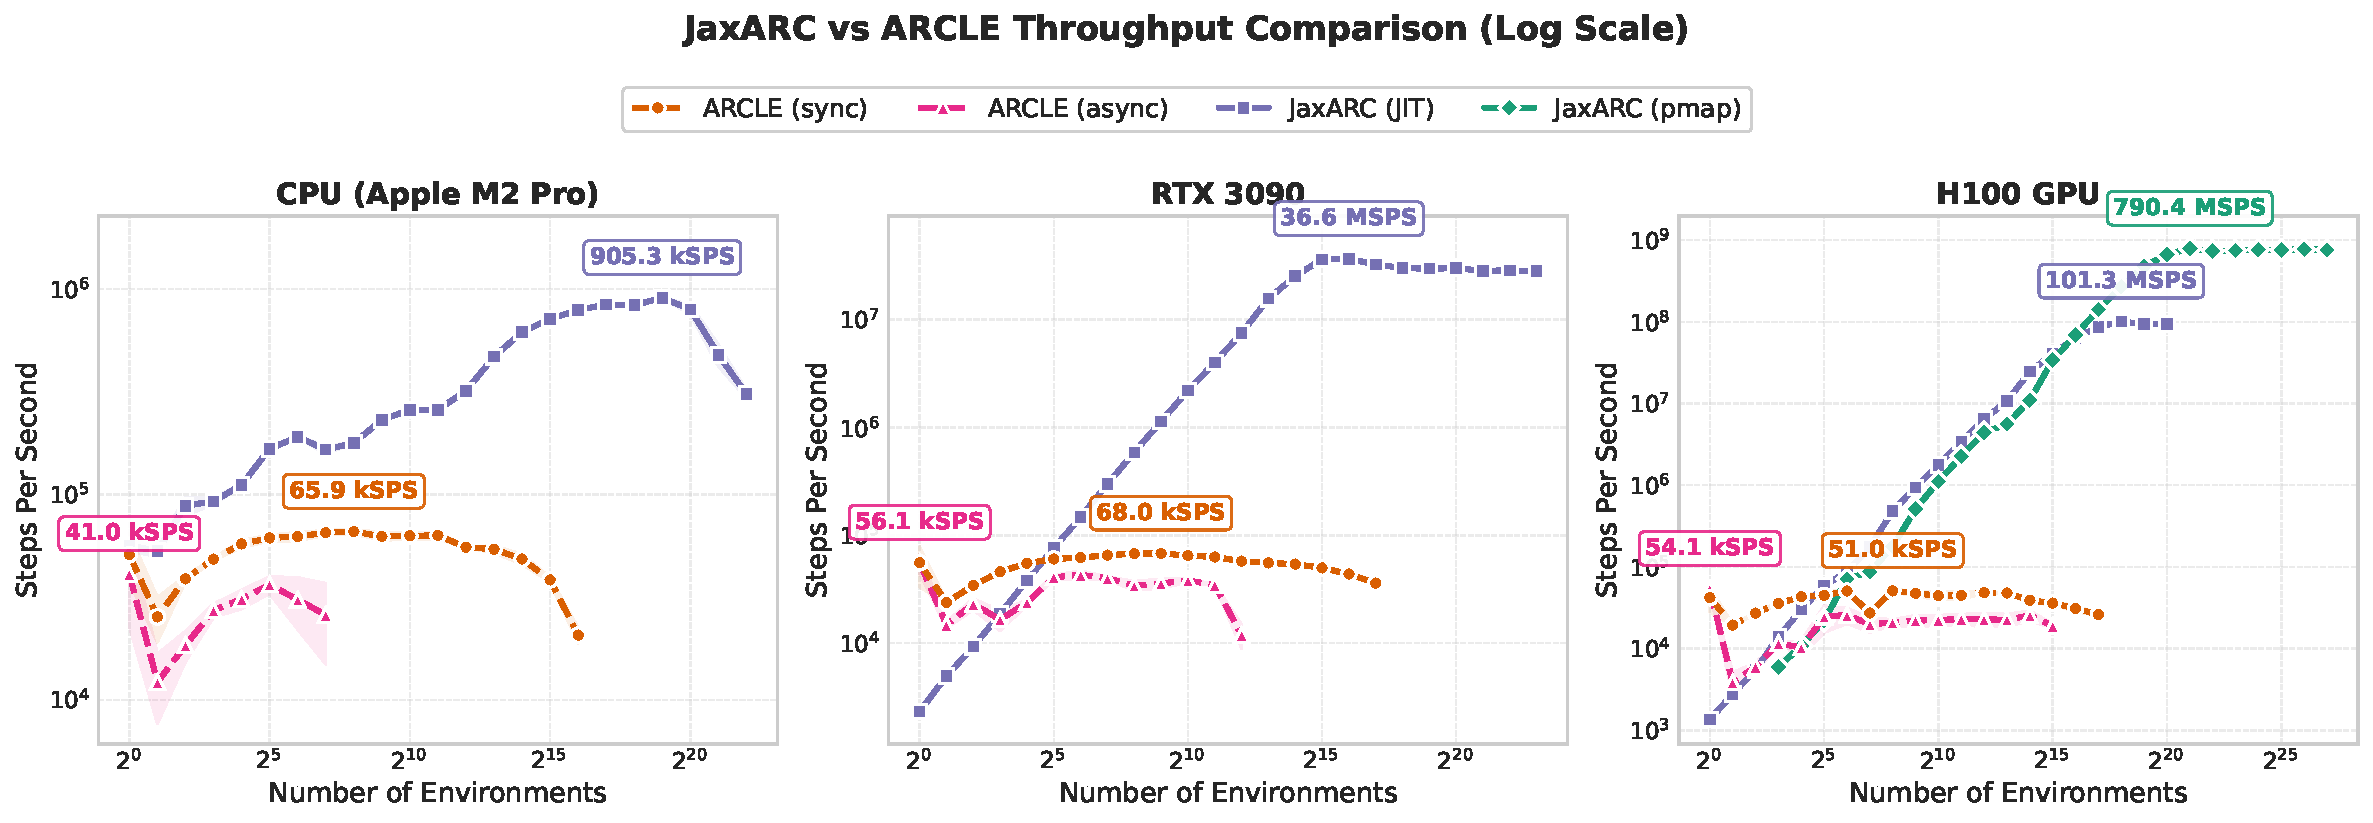
\includegraphics[width=0.95\linewidth]{Figures/throughput_combined_log.pdf}
\caption{Log-scale throughput across hardware platforms. The log scale reveals the crossover point where accelerator-native batching amortizes dispatch costs.}
\label{fig:throughput_log_appendix}
\end{figure}

Detailed speedup comparisons for each hardware tier are provided in Tables~\ref{tab:speedup_cpu_m2_pro}, \ref{tab:speedup_rtx_3090}, and \ref{tab:speedup_h100_gpu}. The H100 JIT run continues beyond the largest matched ARCLE batch and peaks at $101.3$M SPS at batch size $262{,}144$. A separate multi-device \texttt{pmap} benchmark reaches $790.4$M SPS at batch size $2{,}097{,}152$ and gives a $5{,}438.8\times$ speedup at the largest ARCLE-matched batch. We report the multi-device numbers separately because they require eight GPUs and are not directly comparable to ARCLE's CPU-only execution model; the matched-batch single-device numbers in the main results table provide the conservative comparison.

\begin{table}[htbp]
\centering
\caption{Detailed speedup comparison on CPU (M2 Pro)}
\label{tab:speedup_cpu_m2_pro}
\small
\begin{tabular}{lrrrrr}
\toprule
Batch Size & JaxARC SPS & Mode & ARCLE SPS & Mode & Speedup \\
\midrule
1 & 56,266 & jaxarc-jit & 50,823 & arcle-sync & 1.1$\times$ \\
2 & 53,035 & jaxarc-jit & 25,299 & arcle-sync & 2.1$\times$ \\
4 & 87,928 & jaxarc-jit & 38,816 & arcle-sync & 2.3$\times$ \\
8 & 92,525 & jaxarc-jit & 48,384 & arcle-sync & 1.9$\times$ \\
16 & 111,057 & jaxarc-jit & 57,336 & arcle-sync & 1.9$\times$ \\
32 & 166,687 & jaxarc-jit & 61,319 & arcle-sync & 2.7$\times$ \\
64 & 190,381 & jaxarc-jit & 62,324 & arcle-sync & 3.1$\times$ \\
128 & 165,107 & jaxarc-jit & 65,020 & arcle-sync & 2.5$\times$ \\
256 & 177,682 & jaxarc-jit & 65,871 & arcle-sync & 2.7$\times$ \\
512 & 230,453 & jaxarc-jit & 62,397 & arcle-sync & 3.7$\times$ \\
1,024 & 257,889 & jaxarc-jit & 62,820 & arcle-sync & 4.1$\times$ \\
2,048 & 257,877 & jaxarc-jit & 63,111 & arcle-sync & 4.1$\times$ \\
4,096 & 319,194 & jaxarc-jit & 55,270 & arcle-sync & 5.8$\times$ \\
8,192 & 467,960 & jaxarc-jit & 54,033 & arcle-sync & 8.7$\times$ \\
16,384 & 616,683 & jaxarc-jit & 48,383 & arcle-sync & 12.7$\times$ \\
32,768 & 714,731 & jaxarc-jit & 38,334 & arcle-sync & 18.6$\times$ \\
65,536 & 788,855 & jaxarc-jit & 20,634 & arcle-sync & 38.2$\times$ \\
\bottomrule
\end{tabular}
\end{table}

\begin{table}[htbp]
\centering
\caption{Detailed speedup comparison on RTX 3090}
\label{tab:speedup_rtx_3090}
\small
\begin{tabular}{lrrrrr}
\toprule
Batch Size & JaxARC SPS & Mode & ARCLE SPS & Mode & Speedup \\
\midrule
1 & 2,327 & jaxarc-jit & 56,066 & arcle-async & 0.0$\times$ \\
2 & 4,948 & jaxarc-jit & 23,845 & arcle-sync & 0.2$\times$ \\
4 & 9,282 & jaxarc-jit & 34,396 & arcle-sync & 0.3$\times$ \\
8 & 18,667 & jaxarc-jit & 45,991 & arcle-sync & 0.4$\times$ \\
16 & 38,305 & jaxarc-jit & 55,162 & arcle-sync & 0.7$\times$ \\
32 & 76,158 & jaxarc-jit & 60,394 & arcle-sync & 1.3$\times$ \\
64 & 147,835 & jaxarc-jit & 62,266 & arcle-sync & 2.4$\times$ \\
128 & 299,201 & jaxarc-jit & 65,513 & arcle-sync & 4.6$\times$ \\
256 & 589,248 & jaxarc-jit & 67,777 & arcle-sync & 8.7$\times$ \\
512 & 1,141,716 & jaxarc-jit & 68,011 & arcle-sync & 16.8$\times$ \\
1,024 & 2,205,416 & jaxarc-jit & 65,038 & arcle-sync & 33.9$\times$ \\
2,048 & 4,010,852 & jaxarc-jit & 63,005 & arcle-sync & 63.7$\times$ \\
4,096 & 7,519,602 & jaxarc-jit & 57,698 & arcle-sync & 130.3$\times$ \\
8,192 & 15,672,773 & jaxarc-jit & 55,584 & arcle-sync & 282.0$\times$ \\
16,384 & 25,365,090 & jaxarc-jit & 54,126 & arcle-sync & 468.6$\times$ \\
32,768 & 36,337,555 & jaxarc-jit & 50,002 & arcle-sync & 726.7$\times$ \\
65,536 & 36,570,507 & jaxarc-jit & 43,765 & arcle-sync & 835.6$\times$ \\
131,072 & 32,613,474 & jaxarc-jit & 36,131 & arcle-sync & 902.6$\times$ \\
\bottomrule
\end{tabular}
\end{table}

\begin{table}[htbp]
\centering
\caption{Detailed speedup comparison on H100 GPU}
\label{tab:speedup_h100_gpu}
\small
\begin{tabular}{lrrrrr}
\toprule
Batch Size & JaxARC SPS & Mode & ARCLE SPS & Mode & Speedup \\
\midrule
1 & 1,359 & jaxarc-jit & 54,082 & arcle-async & 0.0$\times$ \\
2 & 2,776 & jaxarc-jit & 19,375 & arcle-sync & 0.1$\times$ \\
4 & 5,482 & jaxarc-jit & 27,123 & arcle-sync & 0.2$\times$ \\
8 & 13,912 & jaxarc-jit & 35,775 & arcle-sync & 0.4$\times$ \\
16 & 30,045 & jaxarc-jit & 43,116 & arcle-sync & 0.7$\times$ \\
32 & 59,176 & jaxarc-jit & 44,860 & arcle-sync & 1.3$\times$ \\
64 & 86,458 & jaxarc-jit & 50,575 & arcle-sync & 1.7$\times$ \\
128 & 176,671 & jaxarc-jit & 27,236 & arcle-sync & 6.5$\times$ \\
256 & 482,233 & jaxarc-jit & 51,035 & arcle-sync & 9.4$\times$ \\
512 & 942,287 & jaxarc-jit & 47,571 & arcle-sync & 19.8$\times$ \\
1,024 & 1,766,400 & jaxarc-jit & 44,436 & arcle-sync & 39.8$\times$ \\
2,048 & 3,448,222 & jaxarc-jit & 44,965 & arcle-sync & 76.7$\times$ \\
4,096 & 6,440,953 & jaxarc-jit & 48,389 & arcle-sync & 133.1$\times$ \\
8,192 & 10,743,903 & jaxarc-jit & 47,972 & arcle-sync & 224.0$\times$ \\
16,384 & 24,598,104 & jaxarc-jit & 39,065 & arcle-sync & 629.7$\times$ \\
32,768 & 40,676,131 & jaxarc-jit & 36,002 & arcle-sync & 1129.8$\times$ \\
65,536 & 69,422,302 & jaxarc-pmap & 31,038 & arcle-sync & 2236.7$\times$ \\
131,072 & 141,892,015 & jaxarc-pmap & 26,089 & arcle-sync & 5438.8$\times$ \\
\bottomrule
\end{tabular}
\end{table}

\section{Extended baseline results}
\label{app:extended_baselines}

The extended baseline figures separate shaped editing progress from exact task solving. Episodic return increases on several ARC-AGI and ConceptARC subsets, especially for PPO, but exact success remains substantially lower. This gap indicates that the agents often learn partial edits, reward-shaping behavior, or frequent submissions without reliably producing the full target grid.

Across ARC-AGI groupings, PPO is strongest, REINFORCE is usually the closest competitor, and the value-based methods remain lower or less stable across most panels. ConceptARC shows larger variation across concept groups. Count is the clearest positive case for the shallow-CNN policy-gradient agents, while DDQN shows an early shaped-return gain on Count that does not persist through the full run. Several other groups show moderate shaped return with much weaker exact success. These per-family curves are therefore more informative than a single aggregate score, which would mix qualitatively different learning regimes.

The success-rate panel (Figure~\ref{fig:combined_success_rate}) is the strict measure consistent with the official ARC scoring rule. Reading it together with the episodic-return panels makes the gap between shaping progress and exact submission visible at the per-subset level, and clarifies which subsets remain open problems even for algorithms whose shaped return curves trend upward.

\begin{figure}[htbp]
\centering
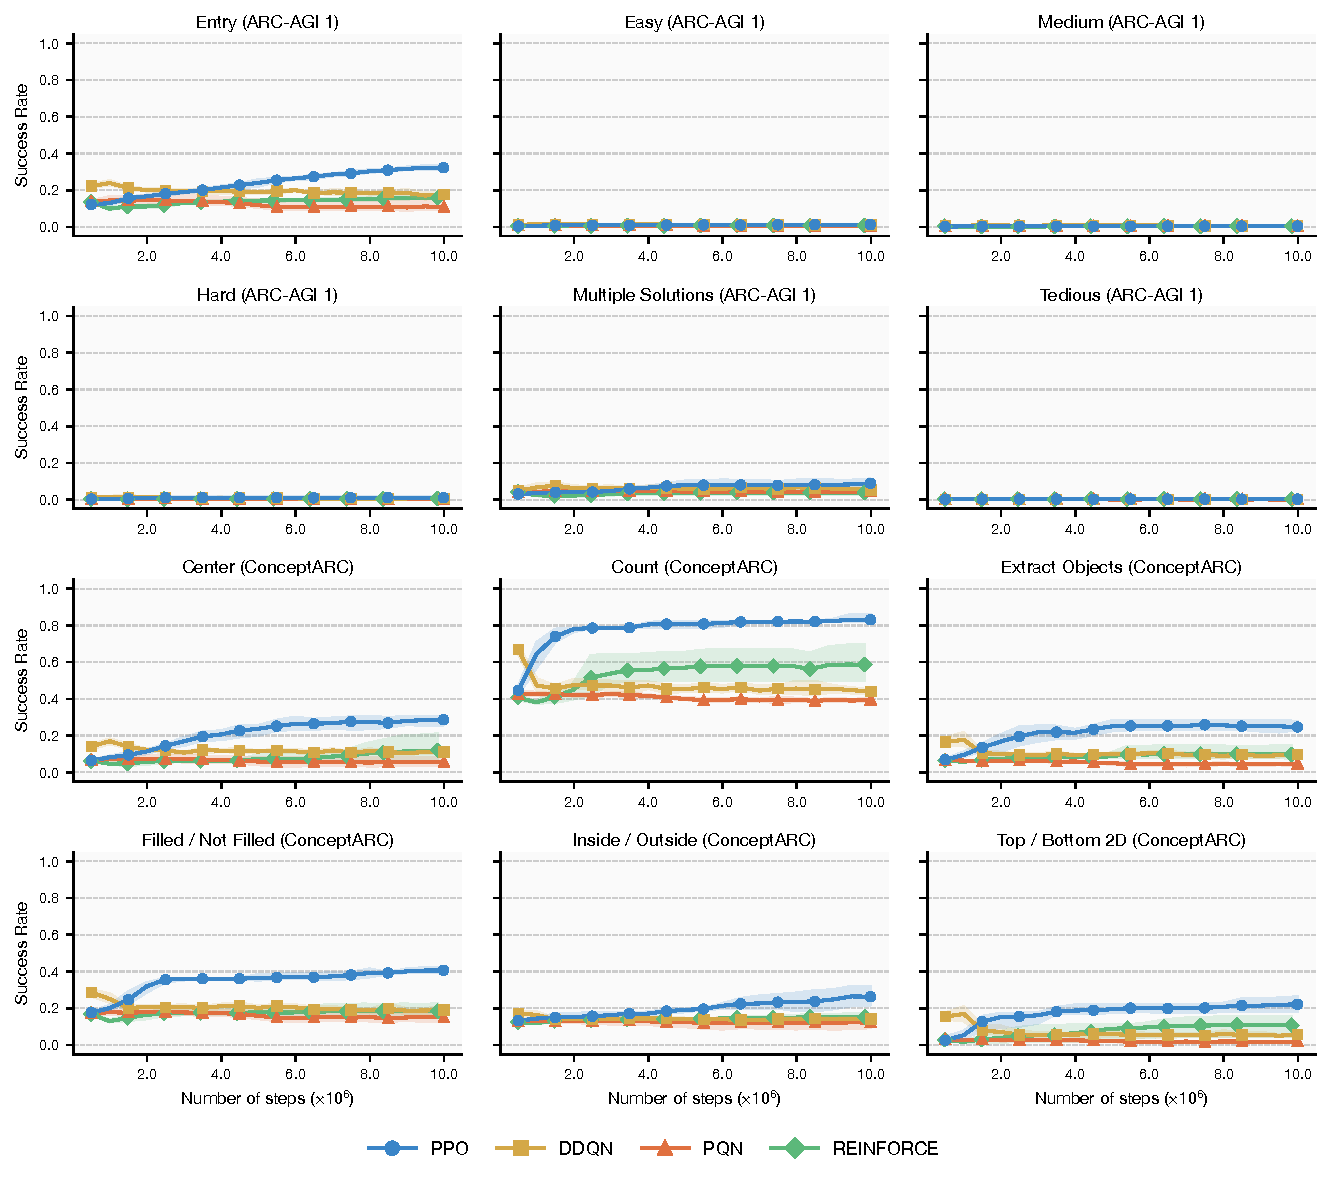
\includegraphics[width=0.95\linewidth]{Figures/combined_success_rate.pdf}
\caption{Success rates across the baseline sweep. Success is a binary, pixel-perfect metric and is significantly harder than optimizing shaped return.}
\label{fig:combined_success_rate}
\end{figure}

\begin{figure}[htbp]
\centering
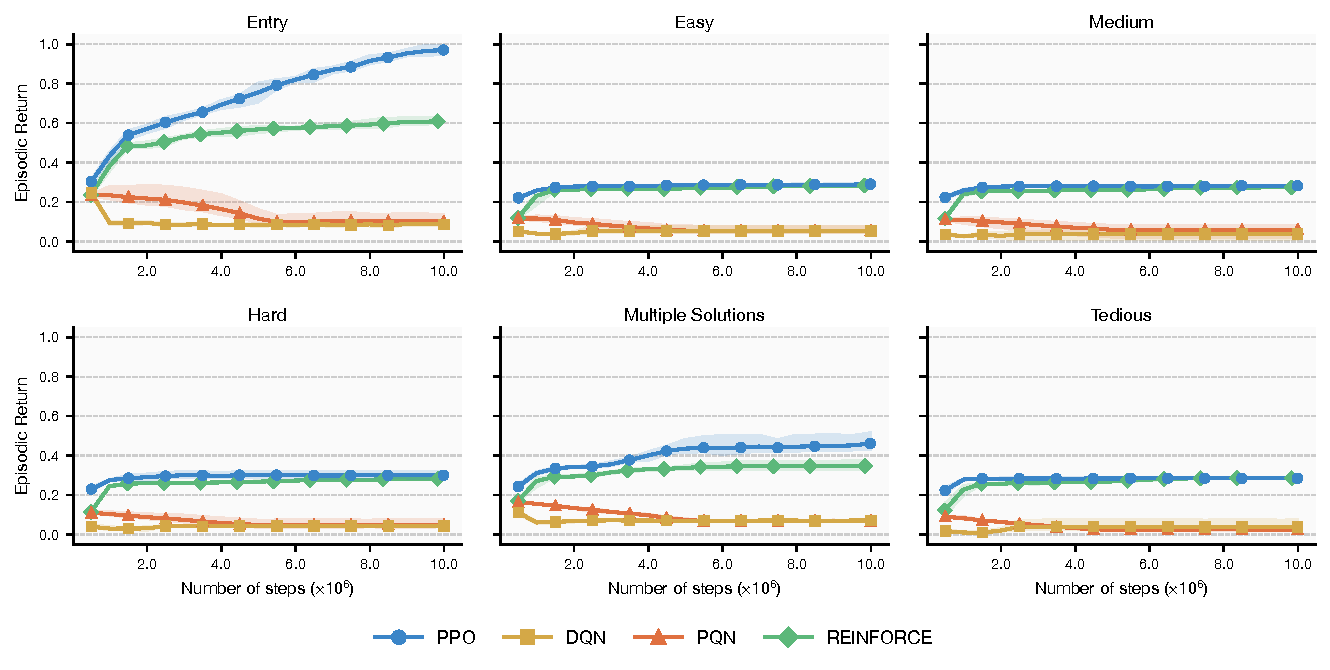
\includegraphics[width=0.95\linewidth]{Figures/arcagi1_episode_return.pdf}
\caption{Episodic return across ARC-AGI-1 groupings. The grouping names are subjective ARC-Game labels rather than official ARC-AGI difficulty levels.}
\label{fig:agi1_episode_return_full}
\end{figure}

\begin{figure}[htbp]
\centering
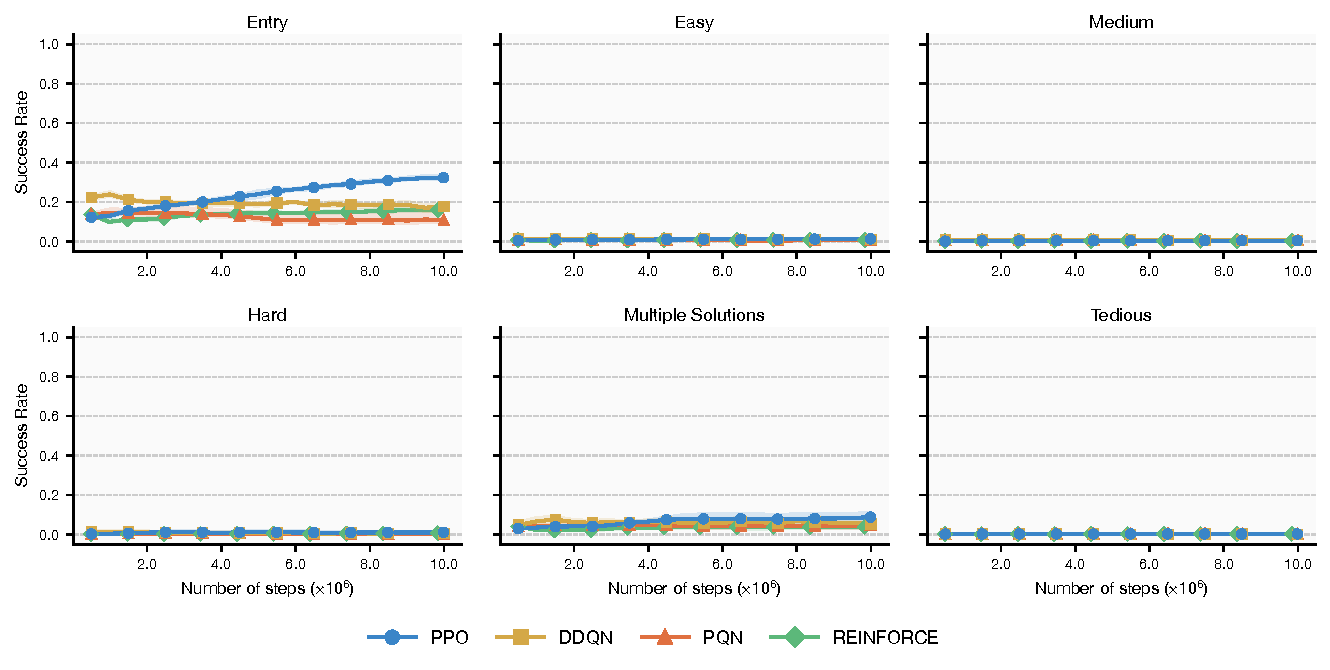
\includegraphics[width=0.95\linewidth]{Figures/arcagi1_success_rate.pdf}
\caption{Success rate across ARC-AGI-1 groupings.}
\label{fig:agi1_success_rate_full}
\end{figure}

\begin{figure}[htbp]
\centering
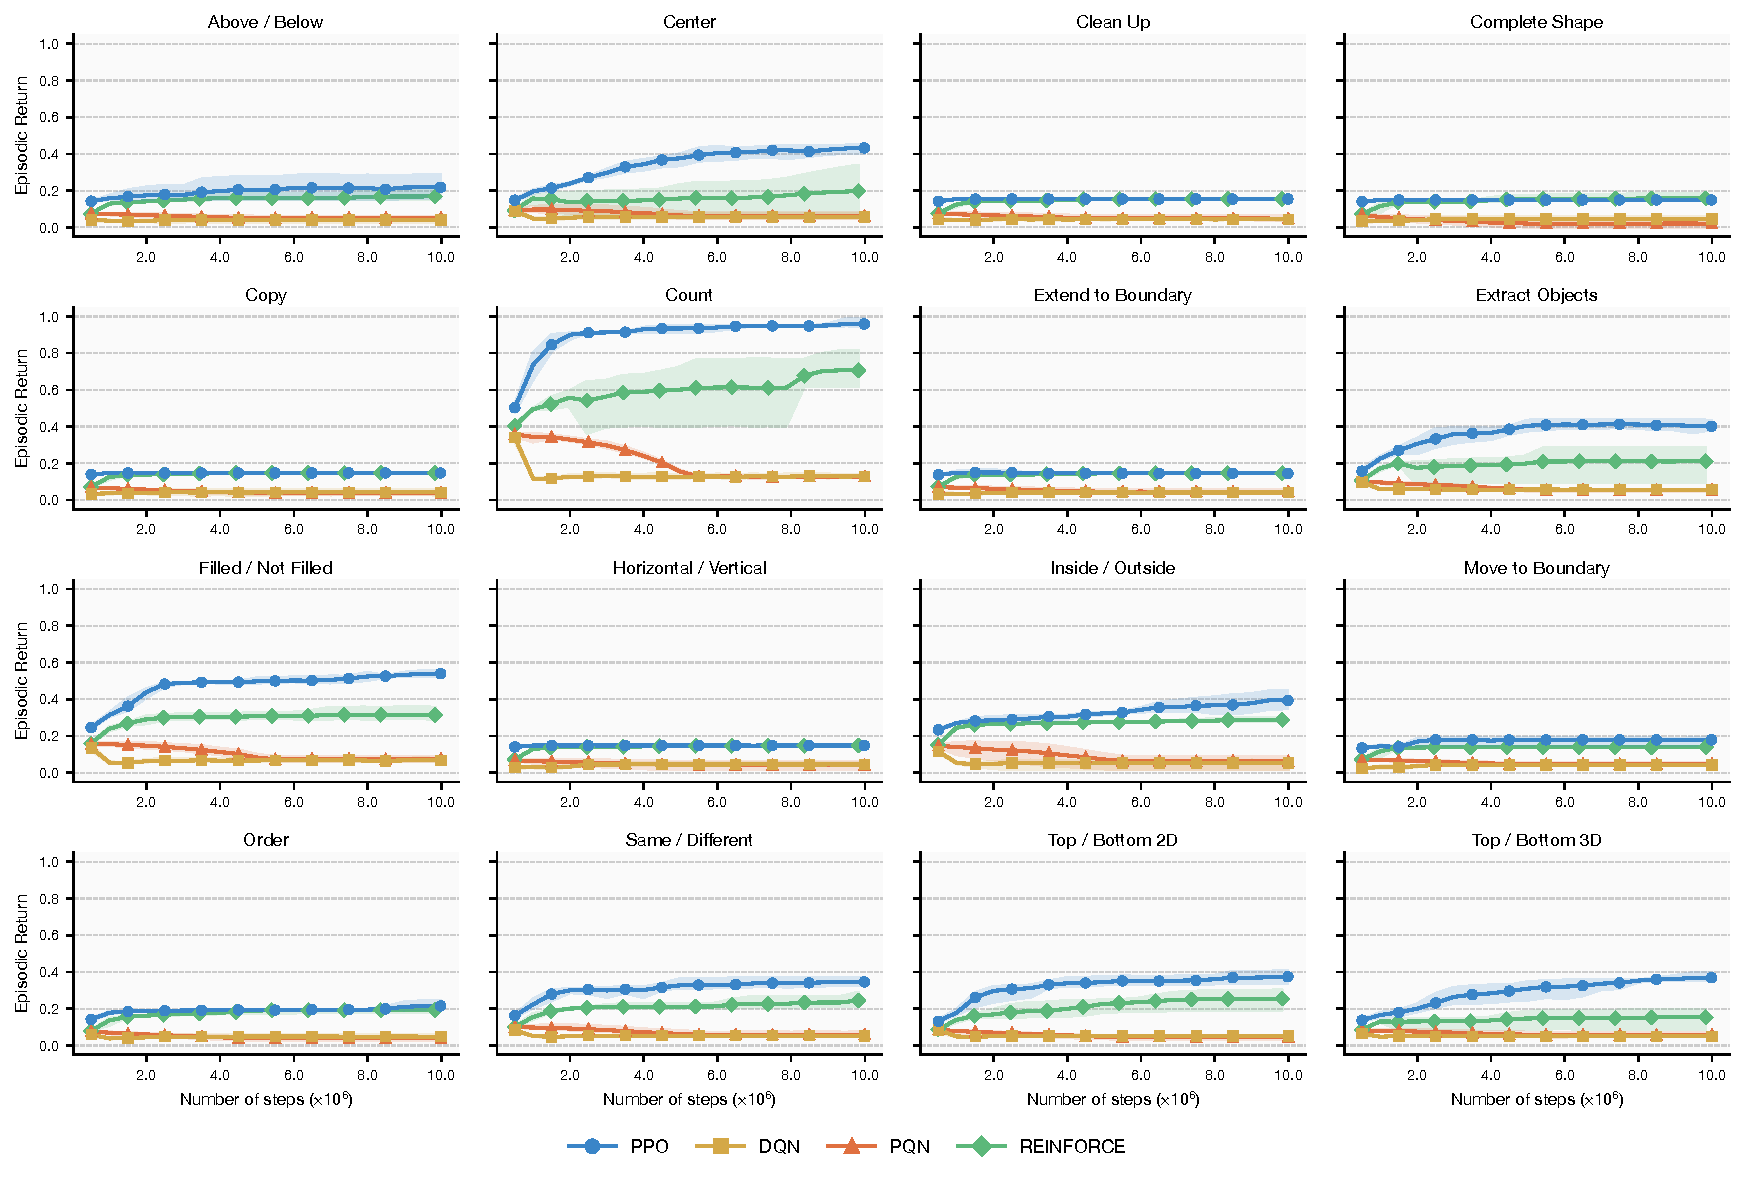
\includegraphics[width=0.95\linewidth]{Figures/conceptarc_episode_return.pdf}
\caption{Episodic return across all 16 ConceptARC concept groups.}
\label{fig:concept_episode_return_full}
\end{figure}

\begin{figure}[htbp]
\centering
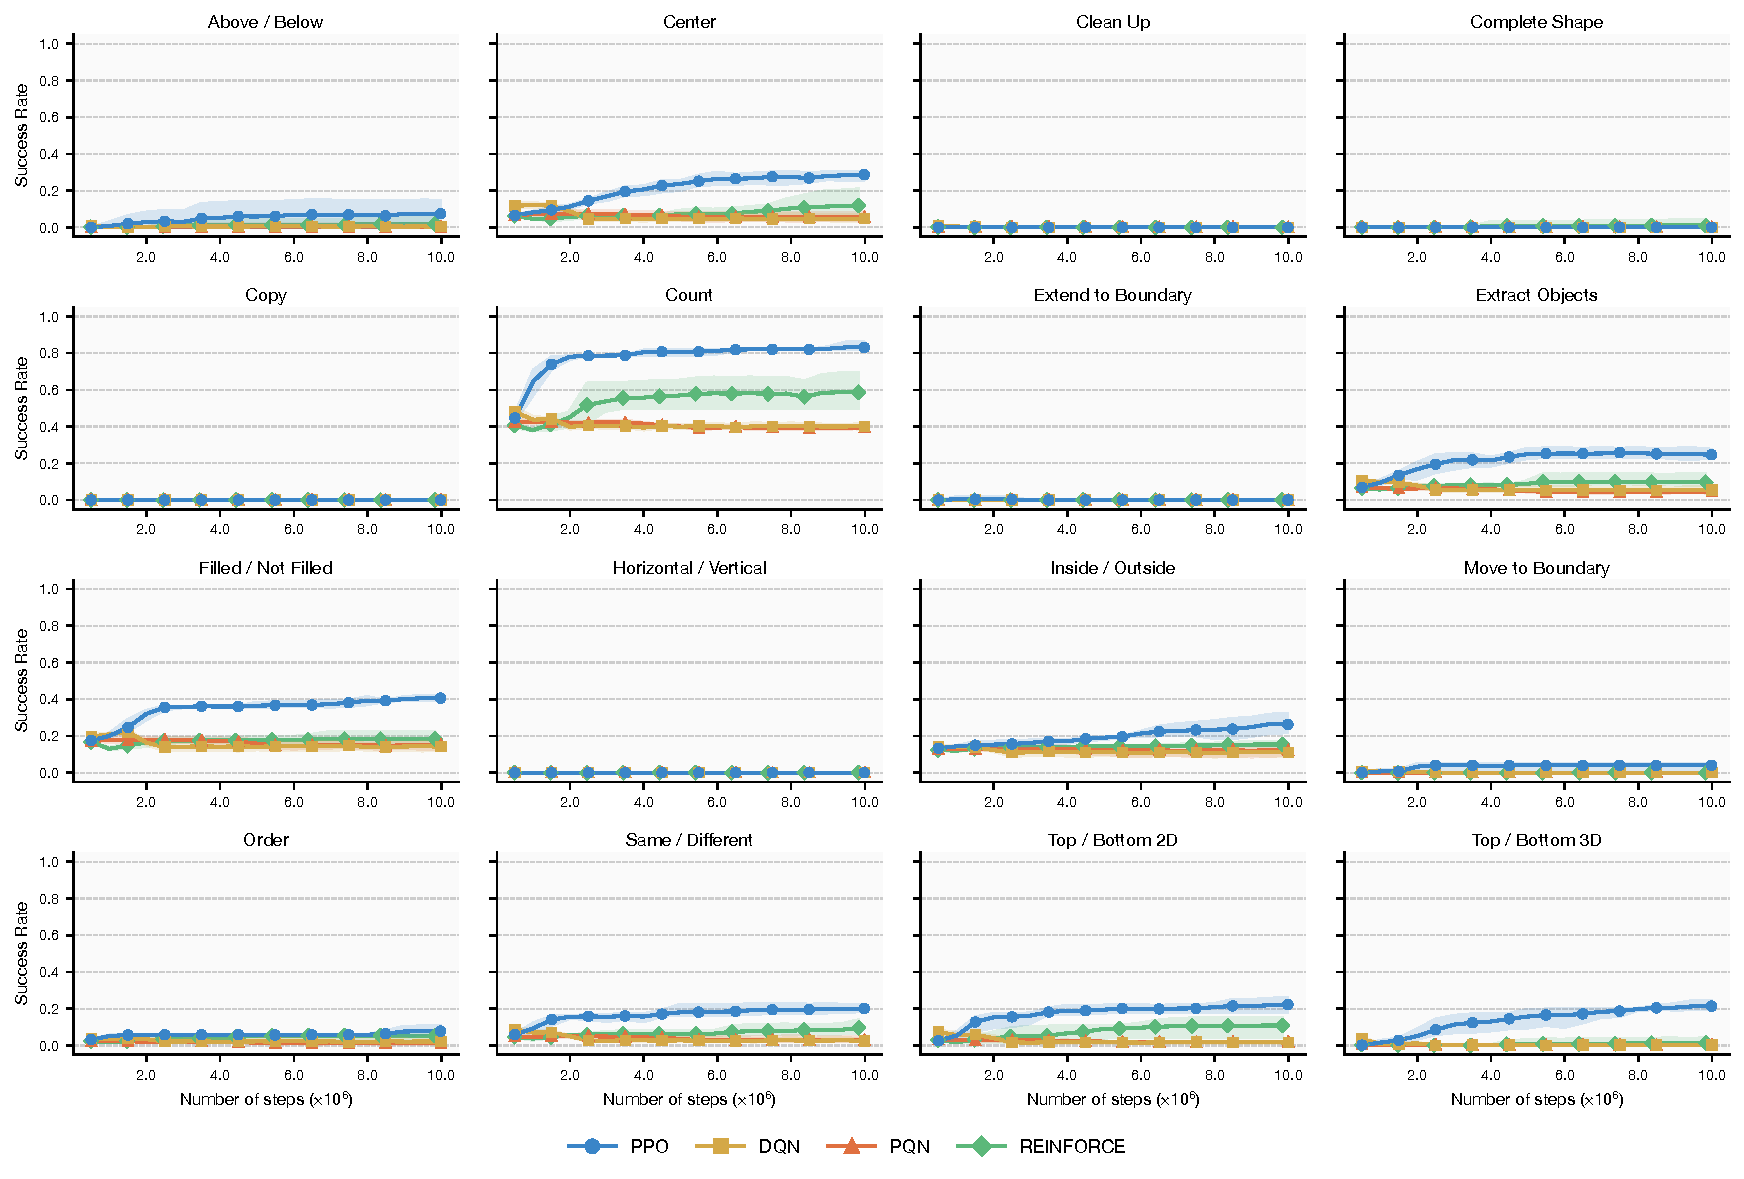
\includegraphics[width=0.95\linewidth]{Figures/conceptarc_success_rate.pdf}
\caption{Success rate across all 16 ConceptARC concept groups.}
\label{fig:concept_success_rate_full}
\end{figure}
\FloatBarrier
